\documentclass[11pt,a4paper,oneside]{article}
\usepackage[utf8x]{inputenc}
\usepackage[francais]{babel}
\usepackage{ucs}
\usepackage{amsmath}
\usepackage{amsfonts}
\usepackage{amssymb}
\usepackage[a4paper]{geometry}
\usepackage{verbatim} 
\usepackage{graphicx}
\usepackage{multirow}
\usepackage{moreverb} 
\geometry{hscale=0.75,vscale=0.85,centering}
\title{GPASA \\ Générateur Pseudo-Aléatoire de Scénario d'Aventure}			
\author{Samuel Lepetit \& Sarkis Mouradian \& Alexandre Lopes-Meda \& Maxime Lefèvre}
\date{Juin 2011}
 
\begin{document}

\maketitle
\tableofcontents
\section{Introduction}
\subsection{Présentation du sujet}
L'objectif de ce projet tutoré était de réaliser un "générateur pseudo-aléatoire de scénarios d'aventure". L'idée est donc d'implémenter un jeu du type "Jeu dont vous êtes le héros", où l'utilisateur (le joueur) se voit proposer des questions, auxquelles il doit répondre: le programme se charge donc ensuite de trouver une autre question à laquelle le joueur doit répondre, qui est tirée dans un ensemble de questions possibles en fonction de ce que le joueur à répondu.

\subsection{Organisation du groupe}
Le Générateur Pseudo-Aléatoire de Scénario d'Aventure ne s'est pas formé en un jour.
Une équipe de quatre personnes composé de Samuel Lepetit, Alexandre Lopes-Meda, Sarkis Mouradian et Maxime Lefevre en est l'origine.

%//raison du choix de ce projet parmis d'autres
\begin{itemize}

\item Plusieurs projets semblaient intéressants, il y avait bien le moteur 3D à la "Doom", un programme permettant de gérer les absences en Amphithéâtre
 et notre générateur pseudo aléatoire de scénario d'aventure.
 Pour certains le moteur 3D était un projet trop commun, pour d'autre le programme gérant les absences n'était tout simplement pas intéressent, le générateur paru comme un choix satisfaisant tout le monde.
Le coté gestion de l'aléatoire fut très intéressant. Comment combiner l'aléatoire dans un jeu avec la cohérence que le scénario de ce jeu implique. C'est cette problématique qui fit pencher notre choix vers ce projet.

%//premiere réunion : création de l'uml diagramme de classe

\item Dès le premier rendez-vous, quelques questions se posèrent.
Qui sera le chef de projet? Dans quel langage sera codé le projet? Comment allons nous répartir les taches?
Il fut très vite convenu  que toutes les décisions seraient prises en groupe et le langage serait le c++ car c'est le langage le plus pratiqué par chacun des membres du groupes et donc le plus maitrisé. Pour répartir les taches, il parait logique qu'il faut d'abord avoir des taches a effectué. C'est ainsi que comme tout réel projet, nous avons réfléchie au code avant de codé. Un diagramme de classe fut élaborer et qui par la suite fut sans cesse mis a jour.
La base des différentes classes que nous avions établie fut rapidement codé. Mais il restait encore le gros du travail, l'algorithme de l'aléatoire et divers questions sur l'implémentation du jeu.

%//réunion discussion structure du projet

\item Il aura bien fallu trois réunions pour ce mettre d'accord sur la structure que vas adopter le Générateur Pseudo Aléatoire de Scénario d'Aventure.


\item La  problématique était d'arriver à une structure facilitant la partie aléatoire de l'implémentation, tout en permettant de garder un jeu cohérent sous tout point de vue.
Qui dit aléatoire, dit arbre binaire ou divers choix possible. Donc la structure doit pouvoir adopter la possibilité d'offrir plusieurs chemins, plusieurs choix.


\item \textbf{Solution trouvée: une structure composée de sous structures.}


A première vu, cette solution parait suffisante et efficace. la décomposition en plusieurs sous-structures permet de briser un de nos principaux problème, la linéarité du jeu. Il faudrait imaginer les sous-structures comme des chemins différents possibles pour le joueur. La partie implémentation aléatoire du programme se charge d'établir la route entre ces divers sous-structures, nous ne rentrerons pas dans les détails ici.


\item Très vite, nous nous sommes rendu compte que décomposer le squelette du jeu en sous-structure ne suffisait pas pour arriver à donner l'illusion d'un jeu aléatoire au joueur. les possibilités offertes par les sous-structures étaient très intéressante mais pas assez.


\item Ce qui nous a paru vite évident, se reposant sur le même principe, c'est le besoin de décomposer les structures en sous-structures qui eux même sont décomposer en sous-structures. Plus le degré de profondeur des sous-ensembles est important, plus les chemins sont variés et l'illusion de l'aléatoire présente. Mais aussi plus c'est profond, plus l'implémentation devient complexe et périlleux.

%//réunion d'apres discution algorithmique sur aléatoire

\item Plusieurs réunions se sont aussi porté sur la mise en place de l'aléatoire dans le jeu. Ce n'était pas une notion simple, il y a eu beaucoup de divergences et de mal à assimiler le concept finale. 
Divers hypothèses on étaient mis en places: 
  \begin{itemize}
  \item Un scénario avec un début fixe, un parcours aléatoire et une fin fixe.
  \newline
  problème: ramener le joueur a la seule fin du jeu prévu
  \item Un scénario avec des étapes obligatoires dans le parcours du joueur
  \newline
  problème: une partie de l'aléatoire du jeu est retiré
  \item Un scénario avec un début fixe et tout le reste aléatoire, la fin compris.
  \newline
  C'est ce qui sera retenu par le groupe.
  \end{itemize}
%//réunion d'apres discution sur Zone questions

Autre décision importante qui fut prise, l'organisation entre les zones et les questions.
Plusieurs idées furent proposés: 
\begin{itemize}
\item faire une liste de questions et tiré au sort une question pour la zone.
   problème: garder une cohérence avec la question tiré et la zone
\item faire différentes listes de questions pour chaque monde
   problème: toujours le même problème, les questions sont plus ciblées par rapport au monde, mais un       		   monde est vaste et les incohérences ont une forte probabilité d'apparaitre tout de même.
   
\end{itemize}
 
 
\item \textbf{Solution trouvée:} Chaque zone possède ces propres questions, donc en tombant dans une zone, on ne peut avoir que des questions lié a cette zone qui pourrait tombé, cela fait quelque peu abstraction du concept aléatoire mais c'est bien le seul endroit ou l'aléatoire n'est pas totale.
%//réunion d'apres discution sur choix de scénario/theme 
\newline

Malgré cela, il nous paraissait tout de même important de rendre un minimum aléatoire les questions lié à une zone. C'est un ainsi que l'idée du système de point est venu: chaque réponse possible permet d'accumuler un nombre de point positif ou négatif. Et en fonction du nombre de point une question est susceptible d'apparaitre ou non.
\newline

Pour faciliter la cohérence dans la transition entres mondes, nous avons choisis de nous inspirer de l'univers du manga "One Piece". Chaque monde est en faite une ile, donc pour passer de n'importe qu'elle ile à une autre, il suffit tout simplement de prendre la mer.
\newline

Au fur et a mesure des réunions, beaucoup d'idées ont été trouvées mais n'ont pas eu de suite malheureusement faute de temps.
\newline

\begin{itemize}
\item Nous avions pensé faire un système de boss. Un boss qui aurai été un monde à lui seul et dont les différentes zones auraient été les étapes et épreuves à parcourir pour réussir à le vaincre.
  \newline
\item Il n'y a pas de fin "évidente" du jeu, mais juste des fin "game-over" en cours de jeu.
  \newline
\item Un système de points de vie fut imaginé, le joueur possédant son endurance et ses points de vie, mais aussi son nom et prénom. Mais encore une fois, tout cela fut inexploitée faute de temps.
  \newline
\end{itemize}
%//choses discuter et non faitre
\end{itemize}

\section{Choix de programmation/d'implémentation}
\subsection{Choix d'implémentation}

\subsubsection{Organisation générale du jeu}

Concernant l'organisation générale du jeu, nous avons fait les choix suivants:
\begin{itemize}
	\item Je joueur à un point de départ fixe. En effet, celui-ci commence le jeu sur une île à partir de laquelle il pourra se diriger vers les autres îles.
	\item Celui-ci se retrouve dans une zone;
	\item A partir de là, une question est choisie aléatoirement parmi une liste de questions relative à cette zone et les propositions à cette question sont présentées au joueur.
	\item certaines des propositions peuvent ne s'afficher 
	\item Le joueur choisi une des propositions et en fonction de son choix, une des zones cible est choisie aléatoirement parmi la liste de zones relative à la proposition.
	\item Le joueur arrive à nouveau sur une zone ,et à nouveau une question est choisie aléatoirement.   
\end{itemize}
\begin{figure}[h]
	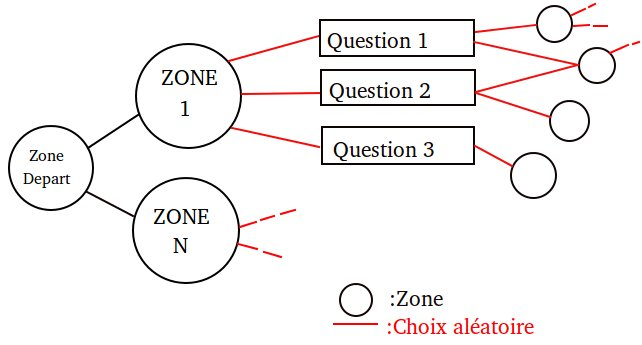
\includegraphics[scale=0.7]{figures/schema-organisation.jpg}
	\caption{Schéma de l'organisation du jeu }
\end{figure}
\subsubsection{Implementation de l'Univers}
Nous avons choisi de représenter l'univers de jeu de la manière suivante:
\begin{itemize}
\item \textbf{Un univers} est constitué d'un ensemble de monde.Il est caractérisé par un nom, mais aussi par sont ensemble de mondes.
\item \textbf{Un monde} est présent dans un Univers et contient lui-meme plusieurs zones. Un monde est caractérisé par un numéro qui lui est propre, par son nom, mais aussi par un ensemble de zones qui le compose. 
\item \textbf{Une Zone} est présente dans un seul et unique monde et celle-ci contient plusieurs questions. Une zone se caractérise par son numéro unique, son som mais aussi un ensemble de questions qui sont liées à cette zone.
\item \textbf{Une question} est relative à une et une seul zone. Celle-ci est caractérisée par: \begin{itemize}
					\item Un nom qui lui est propre.
					\item L'intitulé de cette question qui sera affichée au joueur.
					\item Un ensemble de propositions relatives à cette question.
					\item Le nombre de propositions que cette question possède.
				  \end{itemize} 
\item \textbf{Une proposition} est quand à elle est relative à une et une seule question.
Elle se caractérise par:\begin{itemize}
							\item Le libellé de la proposition qui seras affiché au 									  joueur.
							\item Le nombre de point que rapporte la proposition si 		   							  celle-ci est choisie.
							\item Le nombre de point minimum pour que la proposition 		   							  s'affiche au joueur.
							\item Le nombre de point maximum à partir duquel la 		                                  proposition ne s'affiche plus au joueur.
							\item Un éventuel lien vers un monde si cette proposition 									  renvoit vers un autre monde. 
							\item Une liste de liens vers différentes zones vers 			   							  lequels peut renvoyer la proposition.
							\item La reponse à la proposition qui serat affichée 	  									  lorsque l'utilisateur selectionneras la proposition.   
					    \end{itemize}
					    
\end{itemize}
Ci dessous, un schéma récapitulatif de l'organisation de l'Univers de Jeu.
\begin{figure}[h]
	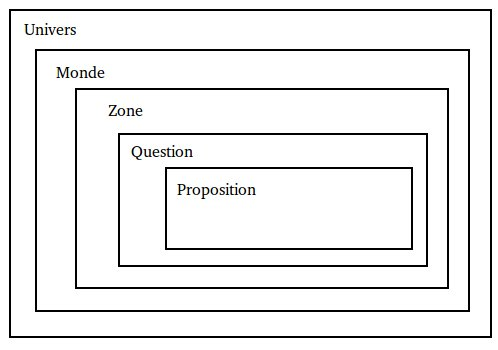
\includegraphics[scale=0.8]{figures/schema-univers.jpg}
	\caption{Schema récapitulatif de l'Organisation de l'Univers de jeu}
\end{figure}
\newpage
\subsubsection{Stockage des questions dans différents dossiers}
Nous avons choisi pour plusieurs raisons(clarté,modulabilité,etc...)d'organiser l'ensemble des fichiers sources du jeu en dossiers et sous-dossiers de la manière suivante:\begin{itemize}
			\item Un dossier par Univers, ici "Univers1" mais nous aurions tout aussi bien en créer plusieurs.
			\item Un dossier par Mondes qui sont contenues dans le fichier de L'Univers. Ici les mondes sont "IleDepart","NorthIsland","WestIsland","SouthIsland" et "EastIsland".
			\item Un dossier par Zones qui sont relatifs au monde au quel elles appartiennent. Le nom de ces dossiers est par exemple "plage","cabane",etc...
			\item Un fichier par question dans chaque dossier de zones.La question dans une zone sera choisie aléatoirement parmi les fichiers présents dans le dossier.   
	     \end{itemize}
\begin{figure}[h]
 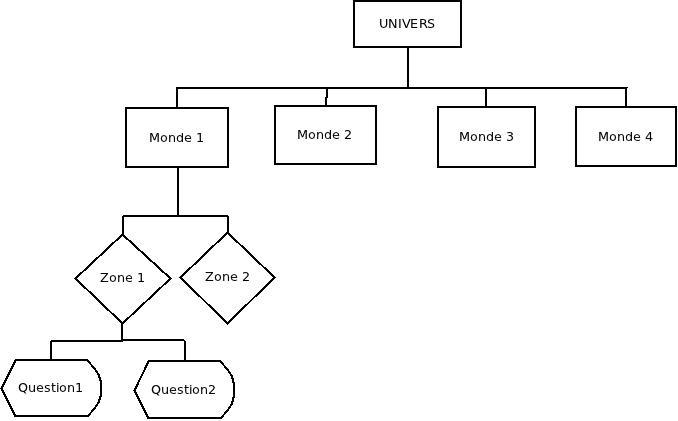
\includegraphics[scale=0.8]{./figures/hier.jpeg}
	\caption{Schéma de l'organisation en dossier }
\end{figure}
\newpage
\subsubsection{Fichier de configuration des questions}
%INTRODUCTION

Les questions utilisées dans le jeux sont, comme nous avons pu le voir, présentes dans plusieurs fichiers texte, un pour chaque question.
\newline
Ces fichiers de questions contiennent non seulement l'intitulé de la dite question, mais aussi les différentes informations qui nous sont nécessaires pour la bonne exécution du jeu. Nous allons voir plus en détail \textbf{l'organisation de ces fichiers de configuration}.
\newline

%FICHIER DE CONFIGURATION

\begin{itemize}

	%INTITULE QUESTION
	\item Une ligne pour l'intitulé de la question
		  
		  \begin{itemize}
		  	\item Celle-ci doit absolument être rédigé sur une seul ligne car nous utilisons la fonctions 				      \textbf{\textit{getline()}} pour récupérer chaque lignes du fichier de question.
		  	
		  	\item Par souci de cohérence, les intitulés de chaque question d'une zone commence par la même     	                         tournure de phrases. Par exemple , pour une zone "fôret", les questions commencerons toutes  	                         par "Vous vous trouvez dans une fôret...." ou une tournure équivalente.
		  \end{itemize}
	
	%PROPOSITION	
	\item Une ligne pour la première proposition
			
		  \begin{itemize}
		  	\item Elle doit être comme pour la question rédigée en une seul ligne
		  \end{itemize}
		  
	%LE NOMBRE DE POINT DE LA PROPOSITION
	\item Le nombre de points que rapporte la proposition
			
		  \begin{itemize}
		  	\item Il est fixé par le rédacteur de la question en fonction des objectif de points à atteindre
		  \end{itemize}
	
	%LA REPONSE
	\item La réponse à la proposition
			
		  \begin{itemize}
		  	\item Cette réponse est affichée lorsque l'utilisateur sélectionne la proposition. Cela permet de lui 						  indiquer la conséquence de son choix.
		  \end{itemize}
	
	%POINTS MINIMUMS
	\item Le nombre de points minimum
			
		  \begin{itemize}
		  	\item Ce nombre de points est celui nécessaire pour que la proposition s'affiche. 
		  	\item Cela est utile pour dans les cas ou l'on veut qu'une action se révèle au héros exclusivement  si 					      celui-ci est passer par certains endroits du monde. 
		  \end{itemize}	
	
	
	%POINTS MINIMUMS
	\item Le nombre de points maximum
			
		  \begin{itemize}
		  	\item Ce nombre de points est basé sur le même principe que pour les point minimum. Mais cette fois-ci, ce 				  nombre de points fixe un seuil à partir duquel la proposition ne s'affiche plus.
		  	\item Cela permet par exemple d'afficher une proposition à son arrivée sur un monde et ne plus l'afficher
		  		  à nouveau si celui-ci revient sur la zone de départ. 
		  \end{itemize}	
		  
	%Lien MONDE
	\item Le Lien vers un éventuel monde
			
		  \begin{itemize}
		  	\item Ce lien est utile lorsque le héros est sur le point de quitter un monde.
		  	\item On indique le nom du monde de destination en toute lettre et si la zone ne renvois pas vers un 	  	                  monde, le champs reste vide. 
		  \end{itemize}	    
	
	%Lien ZONES
	\item Le lien vers les zones
			
		  \begin{itemize}
		  	\item Ces liens correspondent aux différent zones vers lequelles peut renvoyé cette proposition. Pendant 		              le jeu, une de ces zones est choisie aléatoirement.
		  	\item Le nom de chaque zones cible est mis en colonnes les uns à la suite des autres. 
		  \end{itemize}	  

	%Ligne vide
	\item Une ligne vide
		
\end{itemize}  

On ajoute ensuite une ou plusieurs nouvelle(s) proposition les unes à la suite des autres, puis le fichier \textbf{se termine} par \textbf{deux lignes vides}.
\newpage
Voici un exemple de fichier de question tel qu'il se présente dans le jeu:

\begin{listing}{1}
Vous êtes dans le maison des énigmes. Un vieux pirate bossu vous pose cette question : 
"Qu'entend Sartre par 'l'existence précède l'essence' ?". 
Cette homme n'existe pas à votre connaisance ou pas encore du moins mais 
étant vous même un grand théoricien sur l'existence et l'essence voici ce 
qui vous vient à l'esprit :
L'homme a une nature.
0
T'es fou ou quoi !!!. Allez, on recommence.
0
5000

maisonEnigme

L'homme n'est que son projet.
5
Pas mal petit.
0
5000

maisonEnigme

L'existence n'est qu'une étape vers l'immortalité de l'essence.
0
Faux. Essaie encore.
0
5000

maisonEnigme

Vous partez, une question sur un homme inexistant n'a pas de sens.
0

0
5000

ville


\end{listing}




\pagebreak
\subsection{Choix des langages de programmation, des outils et des bibliothèques utilisées}
Tout d'abord, nous avons choisi pour la programmation d'utiliser le langage C++, pour diverses raisons: tout d'abord, il s'agit d'un langage que nous avons longuement étudié en cours, nous donnant un minimum de connaissance et de maitrise dans ce langage, afin de ne pas perdre de temps dans l'apprentissage en lui même du langage.
\subsubsection{L'utilisation de la bibliothèque standard C++: la STL}
Nous avons choisi pour tout le coeur du programme (c'est à dire tout le programme excepté l'interface graphique) d'utiliser la bibliothèque standard du C++, la STL (Standard template library).

Bien sur, nous avons utilisé std::string  dans le cadre du stockage des chaines de caractères, mais le projet nous a aussi permis d'utiliser les conteneurs standard de la STL, tels std::vector ou std::map, qui sont plus haut niveau que de simples tableaux.

Nous avons choisi d'utiliser cette bibliothèque car celle-ci est disponible dans tout les compilateurs C++ à peut près récents, elle est portable et fonctionne donc sur n'importe quelle plateforme: ce qui nous affranchit donc de la dépendance à une bibliothèque qui nous empêcherait de faire un portage vers une autre plateforme.
\subsubsection{L'utilisation de la bibliothèque/framework Qt}
\begin{figure}[h]
\centering

\includegraphics{figures/Qt.png}
\caption{Logo du framework Qt, par Nokia.}
\label{Logo de Qt}
\end{figure}
Pour l'interface graphique de l'application, nous avons choisi d'utiliser le framework Qt de Nokia, qui propose un ensemble de bibliothèques permettant la conception d'interfaces graphiques en C++ de façon rapide et simple.

Nous avons également choisi d'utiliser Qt pour son coté multi plateforme: Ainsi, la bibliothèque est utilisable sur diverses plateformes: Windows, GNU/Linux, Mac OS, mais aussi Android ou Symbian pour le développement mobile, nous permettant de faire une version fonctionelle sur téléphone mobile, bien que non peaufinée. Par ailleurs, la bibliothèque s'intègre parfaitement dans tout les environnements de bureau (Notamment entre les bureaux Gnome 2/GTK sous Linux, KDE4 sous Linux, Gnome 3), en respectant les HIG (Human Interfaces Guidelines, règles de conception pour les interfaces graphiques ) de chaque interface.

Par ailleurs, pour nos besoins, l'utilisation du framework Qt était la plus appropriée, dans le sens où l'interface graphique a été relativement simple à concevoir, nous laissant plus de temps pour la partie algorithmique du programme.

\begin{figure}[p]
\centering
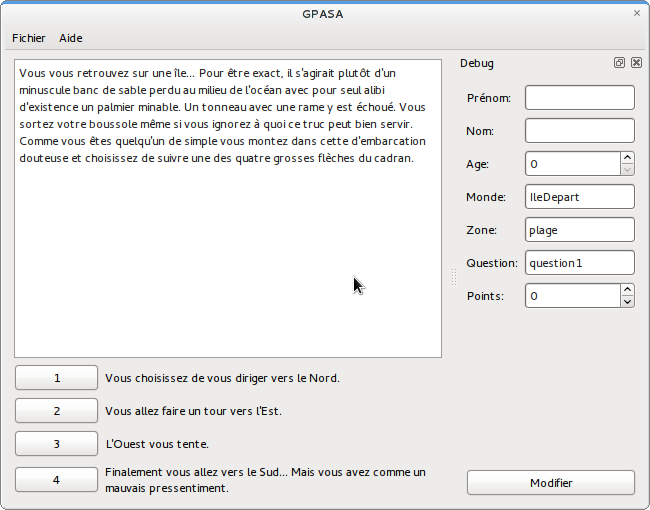
\includegraphics[scale=0.4]{figures/screenshots/gnome3}
\caption{Capture d'ecran de l'application tournant sous un systeme Linux sous Gnome 3.}
\label{CaptureGnome3}
\end{figure}

\begin{figure}[p]
\centering
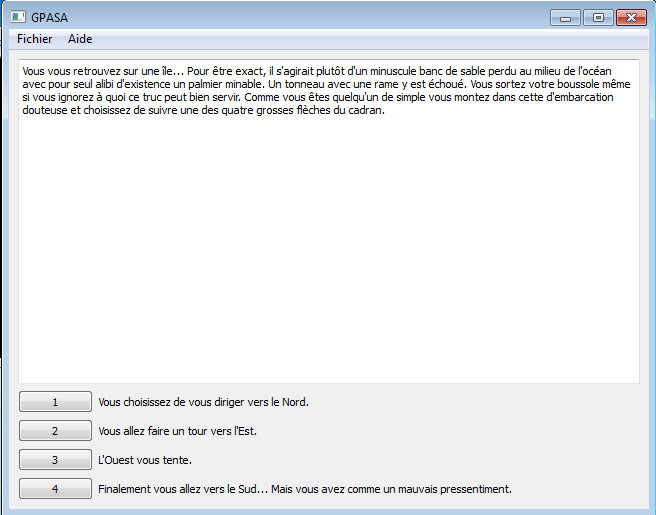
\includegraphics[scale=0.65]{figures/screenshots/windows7}
\caption{Capture d'ecran de l'application tournant sous un systeme Windows 7.}
\label{CaptureWindows7}
\end{figure}



\begin{figure}[p]
\centering
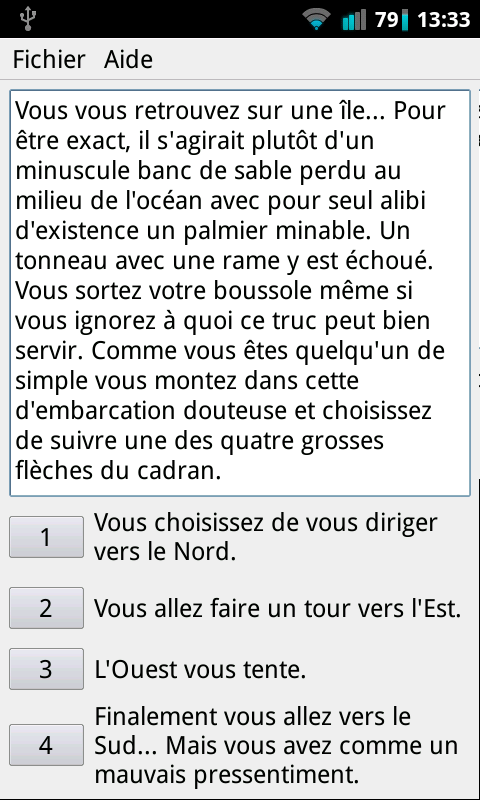
\includegraphics[scale=0.3]{figures/screenshots/androidWVGA}
\caption{Capture d'ecran de l'application tournant sur un téléphone sous Android 2.3.4}
\label{CaptureAndroid}
\end{figure}




\begin{figure}[p]
\centering
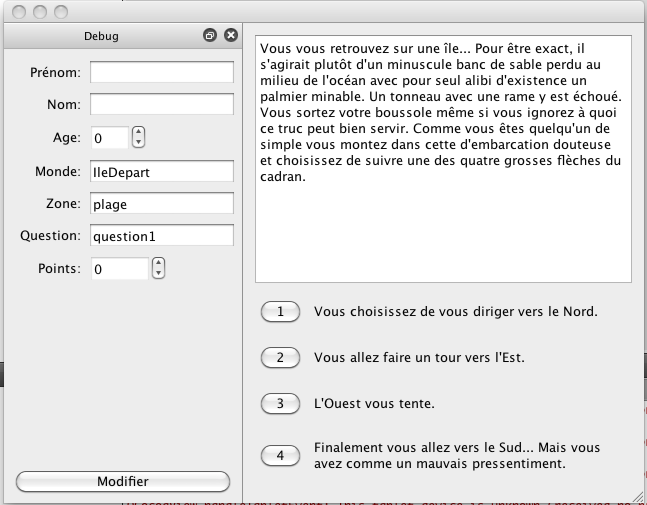
\includegraphics[scale=0.55]{figures/screenshots/OSX}
\caption{Capture d'ecran de l'application tournant sur Mac OS X}
\label{CaptureMac}
\end{figure}

\pagebreak

\subsubsection{L'utilisation d'un gestionnaire de versions: Subversion}

Nous avons choisi pour coordonner notre travail d'utiliser un gestionnaire de versions: Subversion, afin de pouvoir mieux voir les avancements de la programmation et pour pouvoir se coordonner plus facilement, et pour pouvoir mieux voir les changements. Subversion a été choisi préférentiellement à d'autres systèmes de gestion de version (tels git ou mercurial, qui sont plus performants) principalement pour sa simplicité, afin d'éviter un trop apprentissage de l'utilisation du gestionnaire de version, ce qui n'était pas l'objectif.

\subsubsection{La conception du diagramme de classes}
Nous avons choisi d'utiliser l'outil Dia afin de réaliser un diagramme des classes qui nous a permis de penser les différentes classes utilisées par le jeu et nous répartir le travail.

\begin{figure}[h]
\centering
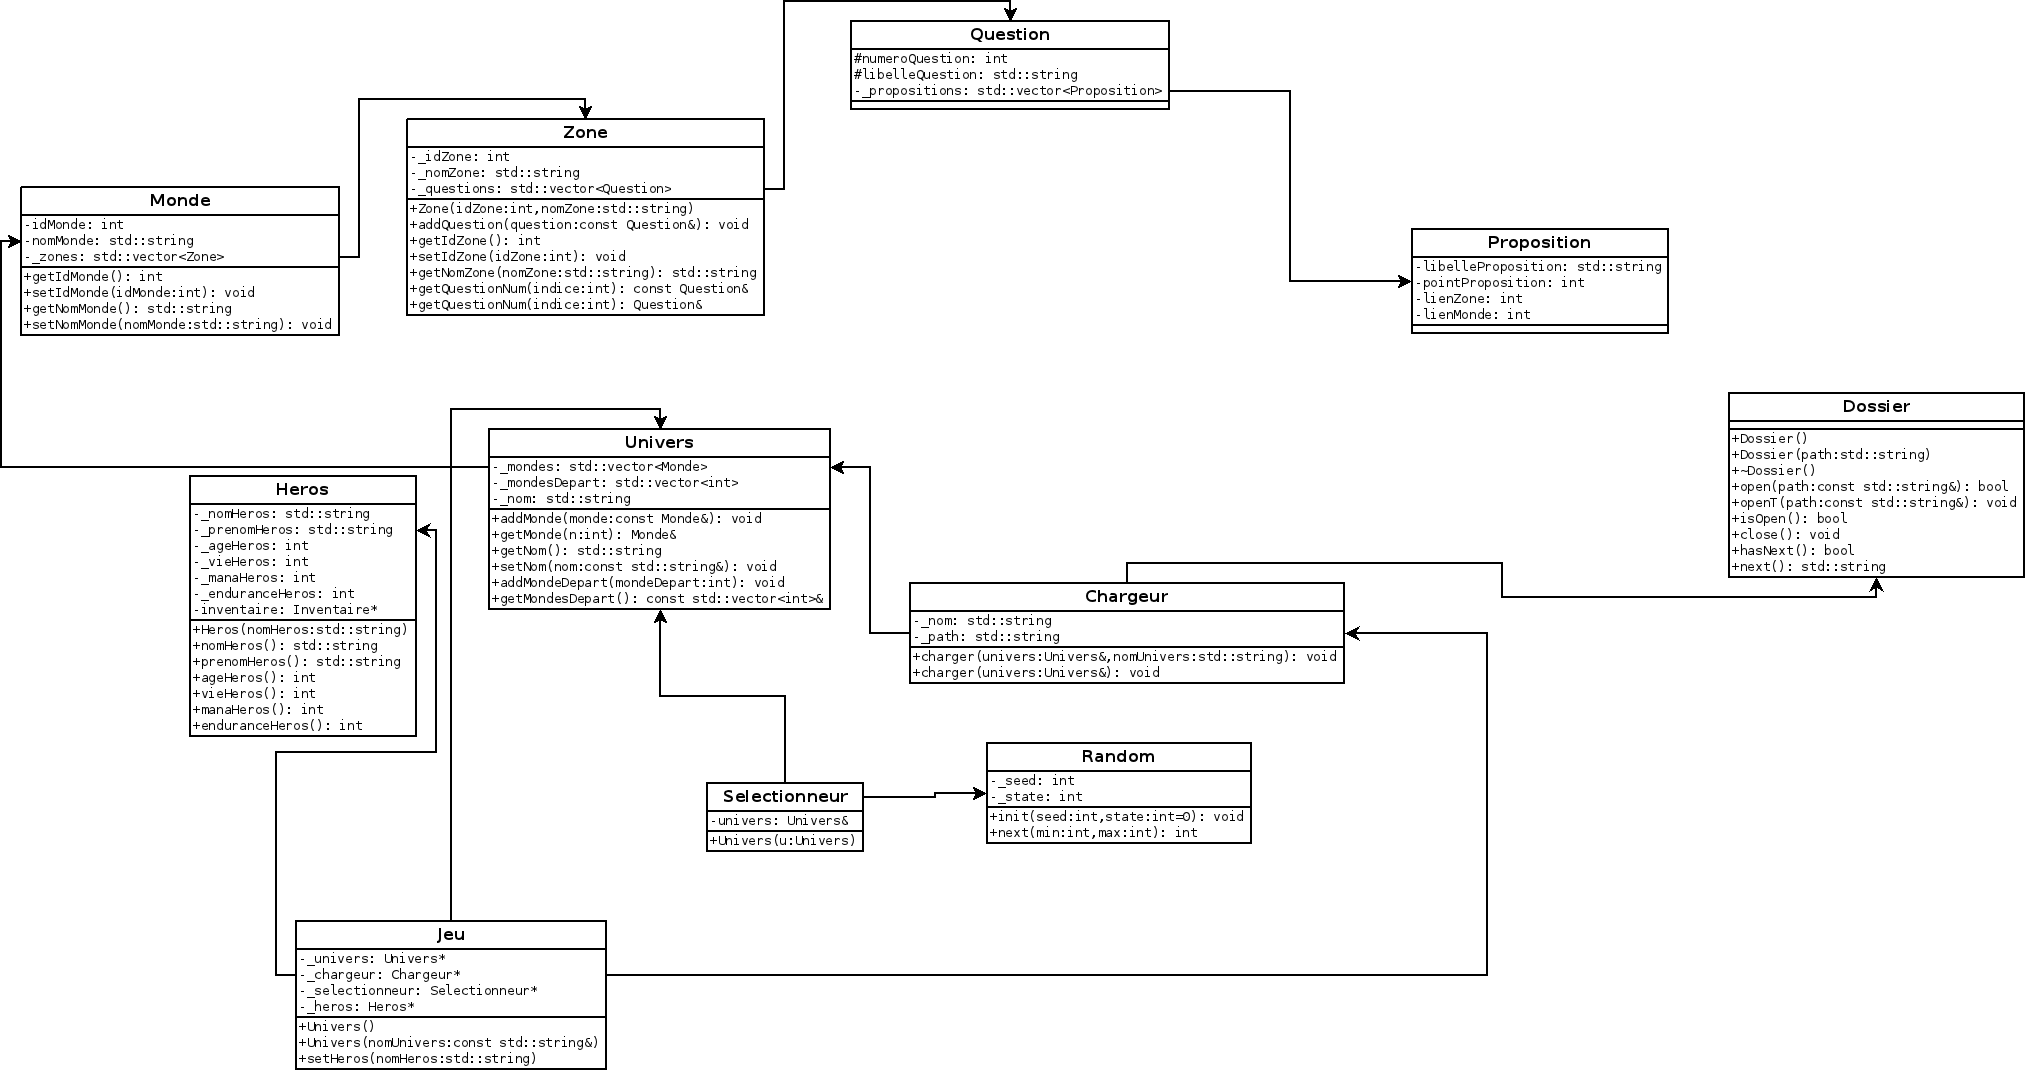
\includegraphics[scale=0.25]{figures/UML.png}
\caption{Partie du diagramme de classe de l'application}
\label{Partie du diagramme de classe de l'application}
\end{figure}


\newpage
\subsection{Choix effectués dans l'implémentation du jeu}
Nous avons choisi de rendre le programme modulaire, de façon à pouvoir facilement changer un module: Ainsi, par exemple, l'interface graphique n'utilise que la classe "Jeu".
\subsubsection{La classe "Random"}
Nous avons choisi de réaliser une abstraction pour le tir des nombres pseudo-aléatoires utilisés dans le jeu pour choisir la prochaine question, ceci nous permettant notamment éventuellement pouvoir nous abstraire des fonctions \textit{rand()} en C, et de proposer des méthodes de plus haut niveau pour tirer des nombres pseudo-aléatoires.

\subsubsection{Les classes "conteneurs": Univers/Monde/Zone/Question/Proposition}
Les classes Univers,Monde,Zone,Question et Proposition sont utilisées afin de stocker les différentes informations de jeu: Chaque classe contient un tableau dynamique (\textit{std::vector}) contenant un élément inférieur (L'univers contient les Mondes, qui contiennent les zones, qui contiennent les questions, etc).

\subsubsection{La classe "Sélectionneur", et son rôle dans le choix des questions}
Nous avons choisi de concevoir une classe "Sélectionneur" pour la sélection de la prochaine question en fonction de la réponse du joueur.

Cette classe procède de la façon suivante: 
\begin{itemize}
	\item Tout d'abord, elle procède à une vérification de la réponse choisie selon plusieurs critères: On prend en compte la cohérence du numéro de réponse choisi (Éviter que le joueur aie répondu à la proposition -1 ou 42 par exemple), et si le joueur est bien dans la fourchette de points nécessaires (Points Minimum $\leq$  Points Joueur $\leq$ Points Maximum 
	\item Ensuite, elle choisit, en fonction de la proposition choisie précédemment, aléatoirement la prochaine zone si celle-ci doit changer. Si un "lien monde" a été renseigné, elle change également le monde actuel.
	\item Enfin, elle tire aléatoirement une question parmi les questions de cette zone.  
\end{itemize}
\subsubsection{La classe Jeu: la liaison avec la/les interfaces graphiques}
L'objectif de la classe "Jeu" est de faire la liaison entre les traitements internes du programme et le reste de l'application (l'interface graphique par exemple).Elle s'occupe ainsi de faire la "glue" entre toutes les autres classes, entre la classe "Héros" gérant le héros, Sélectionneur, et aussi Univers . Également, elle présente  différentes méthodes permettant à l'interface sous-jacente d'avancer dans le jeu, et propage également les exceptions lancées par les classes utilisées.

Elle sert donc d'abstraction pour les classes gérant l'interface graphique.
\subsubsection{La classe "MainWindow", pour l'interface de l'application}
La classe MainWindow  est la classe principale de l'interface graphique. Celle-ci gère toute l'interface graphique du jeu, gérant l'affichage de la question et des boutons, en fonction de la question.

Elle fait la liaison avec les données de jeu en utilisant une instance de la classe "Jeu", qu'elle utilise pour récupérer les différentes informations et renvoyer les valeurs choisies par le joueur.


L'objectif de la classe DebugDock est, quant à lui, à des fins de débogage, d'afficher toutes les informations sur le joueur et l'état actuel, et de pouvoir modifier les informations actuelles. Elle se présente sous la forme d'un "dock" dans l'interface.


\section{Conclusion}



\subsection{Ce qui aurait pu etre amélioré}

Par manque de temps, nous n'avons pu réaliser certaine amelioration du jeu qui auraient permis de le rendre plus complet. Ces améliorations sont les suivantes: 
\begin{itemize}
	\item Les points de vie du héros n'ont pu être implémentés. Actuellement,selon ses choix, le joueur est soit envoyé vers une nouvelle question, soit vers un écran de fin de jeu. Les points de vie auraient permis d'assouplir le gameplay.
	\item Certains attributs comme le nom, le prénom et l'âge du héros, n'ont pas été suffisamment inclus dans le jeu. Le joueur peut bien sûr les renseigner mais ils n'auront pas d'incidences au cours de la partie. À l'origine, nous avions par exemple prévu d'implémenter différentes tranches d'âges ce qui aurait permis de mieux adapter les situations au personnage.
	\item la mise en place d'une sauvegarde qui aurait permis au joueur de reprendre la partie là ou il se serait arrêter.
	\item L'ajout de monstres auquel le joueur serait confronté et en fonction de ses actions, il y aurait une baisse de ses point de vie ou celui du monstre.
	\item Nous aurions pu rajouter un inventaire que le joueur aurait pu consulter en cours de route
	\item La mise en place d'une carte du monde qui indiquerait au joueur où celui-ci se trouve dans le monde.
	\item Le raffinement de l'interface graphique, qui est relativement simple et qui est par exemple relativement peu adaptée aux appareils mobiles, où qui rend assez mal sous Mac OS X.
\end{itemize}
  

 faute de temps, 


\subsection{Conclusion générale}

Ce projet nous a aidé à approfondir les notions liées à la programmation orienté objet en C++.

Par ailleurs, l'utilisation du framework QT a permis une nouvelle approche en matière de création d'interface graphique. L'utilisation de subversion nous a également permis de nous initier aux systèmes de gestion de version.
 
L'importance de ce projet par rapport aux exercices habituels nous a incité à être efficace au possible. Dans cette optique nous avons découvert et utilisé la syntaxte Doxygen pour nos commentaires afin d'obtenir rapidement une documentation complète.

\end{document}